%!TEX program = xelatex
\documentclass[11pt]{beamer}

\usepackage{amsfonts}
\usepackage{amsmath}
\usepackage{blindtext}
\usepackage{enumitem}

\usetheme{SaoPaulo}

\title{Python Basics!}
\subtitle{branched control, range, lists}
\author{CS101 Lecture \#8}
\date{2016-09-19}

\setcounter{showSlideNumbers}{1}

\begin{document}
  \setcounter{showProgressBar}{0}
  \setcounter{showSlideNumbers}{0}

%%%%%%%%%%%%%%%%%%%%%%%%%%%%%%%%%%%%%%%%%%%%%%%%%%%%%%%%%%%%%%%%%%%%%%%%%%%%%%%%
\frame{\titlepage}

%%%%%%%%%%%%%%%%%%%%%%%%%%%%%%%%%%%%%%%%%%%%%%%%%%%%%%%%%%%%%%%%%%%%%%%%%%%%%%%%
\setcounter{framenumber}{0}
\setcounter{showProgressBar}{1}
\setcounter{showSlideNumbers}{1}

%%%%%%%%%%%%%%%%%%%%%%%%%%%%%%%%%%%%%%%%%%%%%%%%%%%%%%%%%%%%%%%%%%%%%%%%%%%%%%%%
\section{Administrivia}

%%%%%%%%%%%%%%%%%%%%%%%%%%%%%%%%%%%%%%%%%%%%%%%%%%%%%%%%%%%%%%%%%%%%%%%%%%%%%%%%
\begin{frame}
  \frametitle{Administrivia}
  \Enlarge
  \begin{itemize}
  \myitem  Homework \#4 is due Friday Sep.\ 23.
  \myitem  Midterm \#1 will be Monday Oct.\ 3.  (evening)
  \end{itemize}
\end{frame}

%%%%%%%%%%%%%%%%%%%%%%%%%%%%%%%%%%%%%%%%%%%%%%%%%%%%%%%%%%%%%%%%%%%%%%%%%%%%%%%%
\section{Warmup Quiz}

%%%%%%%%%%%%%%%%%%%%%%%%%%%%%%%%%%%%%%%%%%%%%%%%%%%%%%%%%%%%%%%%%%%%%%%%%%%%%%%%
\begin{frame}[fragile]
  \frametitle{Question \#1}
  \Enlarge

  \begin{semiverbatim}
s = 'ABCDEFGH'
t = ''
i = 0
while i < 8:
    t = t + s[ i+1 ]
    i += 2
  \end{semiverbatim}
  What is the final value of \texttt{t}?
  \begin{enumerate}[label=\Alph*]
  \item  \texttt{"ACEG"}
  \item  \texttt{"BDFH"}
  \item  \texttt{"ABCDEF"}
  \item  \texttt{"ABEF"}
  \end{enumerate}
\end{frame}

%%%%%%%%%%%%%%%%%%%%%%%%%%%%%%%%%%%%%%%%%%%%%%%%%%%%%%%%%%%%%%%%%%%%%%%%%%%%%%%%
\begin{frame}[fragile]
  \frametitle{Question \#2}
  \Enlarge

  \begin{semiverbatim}
s = '0123456789'
t = ''
i = 0
while i < 5:
    if (i%2) == 1:
        t = t + s[ i-1 ]
    if (i%2) == 0:
        t = t + s[ i+1 ]
    i = i + 1
\end{semiverbatim}
  What is the final value of \texttt{t}?
  \begin{enumerate}[label=\Alph*]
  \item  \texttt{"92143"}
  \item  \texttt{"103254"}
  \item  \texttt{"10325"}
  \item  \texttt{"921436"}
  \item  None (loop doesn't terminate)
  \end{enumerate}
\end{frame}

%%%%%%%%%%%%%%%%%%%%%%%%%%%%%%%%%%%%%%%%%%%%%%%%%%%%%%%%%%%%%%%%%%%%%%%%%%%%%%%%
\section{Conditional Execution}

%%%%%%%%%%%%%%%%%%%%%%%%%%%%%%%%%%%%%%%%%%%%%%%%%%%%%%%%%%%%%%%%%%%%%%%%%%%%%%%%
\begin{frame}[fragile]
  \frametitle{Example:  \texttt{if} statement}
  \Enlarge

  \begin{semiverbatim}
ans = input( "Enter a number:" )
if float(ans) < 0:
    print( "The number was negative." )
  \end{semiverbatim}
\end{frame}

%%%%%%%%%%%%%%%%%%%%%%%%%%%%%%%%%%%%%%%%%%%%%%%%%%%%%%%%%%%%%%%%%%%%%%%%%%%%%%%%
\begin{frame}[fragile]
  \frametitle{Control flow}
  \Enlarge

  \begin{itemize}
  \myitem  \emph{Control flow} represents actual sequence of lines executed by processor. \pause
  \myitem  \emph{Conditional execution} lets you execute (or not) a block of code based on logical comparison.
  \end{itemize}
\end{frame}

%%%%%%%%%%%%%%%%%%%%%%%%%%%%%%%%%%%%%%%%%%%%%%%%%%%%%%%%%%%%%%%%%%%%%%%%%%%%%%%%
\begin{frame}[fragile]
  \frametitle{Branched control flow}
  \Enlarge

  \begin{itemize}
  \myitem  We often need to make decisions with \emph{several} options. \pause
  \myitem  \emph{Branched conditional execution} lets you execute one of several blocks of code.
  \end{itemize}
\end{frame}

%%%%%%%%%%%%%%%%%%%%%%%%%%%%%%%%%%%%%%%%%%%%%%%%%%%%%%%%%%%%%%%%%%%%%%%%%%%%%%%%
\begin{frame}[fragile]
  \frametitle{Example}
  \Enlarge

  \begin{semiverbatim}
def absolute(x):
    if x >= 0:
        return x
    else:
        return -x
  \end{semiverbatim}
\end{frame}

%%%%%%%%%%%%%%%%%%%%%%%%%%%%%%%%%%%%%%%%%%%%%%%%%%%%%%%%%%%%%%%%%%%%%%%%%%%%%%%%
\begin{frame}[fragile]
  \frametitle{\texttt{if}/\texttt{else} statement}
  \Enlarge

  \begin{itemize}
  \myitem  We create an \texttt{if}/\text{else} statement as follows:
    \begin{itemize}
    \mysubitem  the keyword \texttt{if}
    \mysubitem  a logical comparison (results in \texttt{bool})
    \mysubitem  a \textbf{block} of code
    \mysubitem  the keyword \texttt{else}
    \mysubitem  a different \textbf{block} of code
    \end{itemize}
  \end{itemize}
\end{frame}

%%%%%%%%%%%%%%%%%%%%%%%%%%%%%%%%%%%%%%%%%%%%%%%%%%%%%%%%%%%%%%%%%%%%%%%%%%%%%%%%
\begin{frame}[fragile]
  \frametitle{String comparison methods}
  \Enlarge

  \begin{itemize}
  \myitem  These produce Boolean output.
    \begin{tabular}{ll}
    \texttt{isdigit()} & Does a string contain only numbers?
    \texttt{isalpha()} & Does a string contain only text?
    \texttt{islower()} & Does a string contain only lower-case letters?
    \texttt{isupper()} & Does a string contain only upper-case letters?
    \end{tabular}
  \end{itemize}
\end{frame}

%%%%%%%%%%%%%%%%%%%%%%%%%%%%%%%%%%%%%%%%%%%%%%%%%%%%%%%%%%%%%%%%%%%%%%%%%%%%%%%%
\begin{frame}[fragile]
  \frametitle{Example:  String comparison methods}
  \Enlarge

  \begin{semiverbatim}
answer = input( 'How do you feel?  ' )
if not answer.isalpha():
    print( "I don't understand." )
else:
    print( "Ah, you feel %s." % answer )
\end{frame}

%%%%%%%%%%%%%%%%%%%%%%%%%%%%%%%%%%%%%%%%%%%%%%%%%%%%%%%%%%%%%%%%%%%%%%%%%%%%%%%%
\begin{frame}[fragile]
  \frametitle{Sequence operators}
  \Enlarge

  \begin{itemize}
  \myitem  These produce Boolean output.
    \begin{tabular}{ll}
    \texttt{in}     & Is one string inside of the other?
    \texttt{not in} & Is one string not inside of the other?
    \end{tabular}
  \end{itemize}
\end{frame}

%%%%%%%%%%%%%%%%%%%%%%%%%%%%%%%%%%%%%%%%%%%%%%%%%%%%%%%%%%%%%%%%%%%%%%%%%%%%%%%%
\begin{frame}[fragile]
  \frametitle{Example}
  \Enlarge

  \begin{semiverbatim}
def fun(s):
    return s.isalpha() and 'a' in s

x = fun( "sam" ) and fun( "AS" )
  \end{semiverbatim}
  What is the value of \texttt{x}?
  \begin{enumerate}[label=\Alph*]
  \item  \texttt{True}
  \item  \texttt{False}
  \end{enumerate}
\end{frame}

%%%%%%%%%%%%%%%%%%%%%%%%%%%%%%%%%%%%%%%%%%%%%%%%%%%%%%%%%%%%%%%%%%%%%%%%%%%%%%%%
\begin{frame}[fragile]
  \frametitle{Nesting}
  \Enlarge

  \begin{itemize}
  \myitem  Sometimes we need to make more than one decision. \pause
  \myitem  We can \emph{nest} blocks. \pause
    \begin{Verbatim}
word = input( 'Enter a Scrabble word:  ' )
if not word.isalpha():
    print( 'There are only letters in Scrabble!' ) \pause
else:
    if not word.isupper():      # why wouldn't `word.islower()` work?
        word = answer.upper()
    print( 'You entered %s.' % word )
    \end{Verbatim}
  \end{itemize}
\end{frame}

%%%%%%%%%%%%%%%%%%%%%%%%%%%%%%%%%%%%%%%%%%%%%%%%%%%%%%%%%%%%%%%%%%%%%%%%%%%%%%%%
\begin{frame}
  \frametitle{Nesting}
  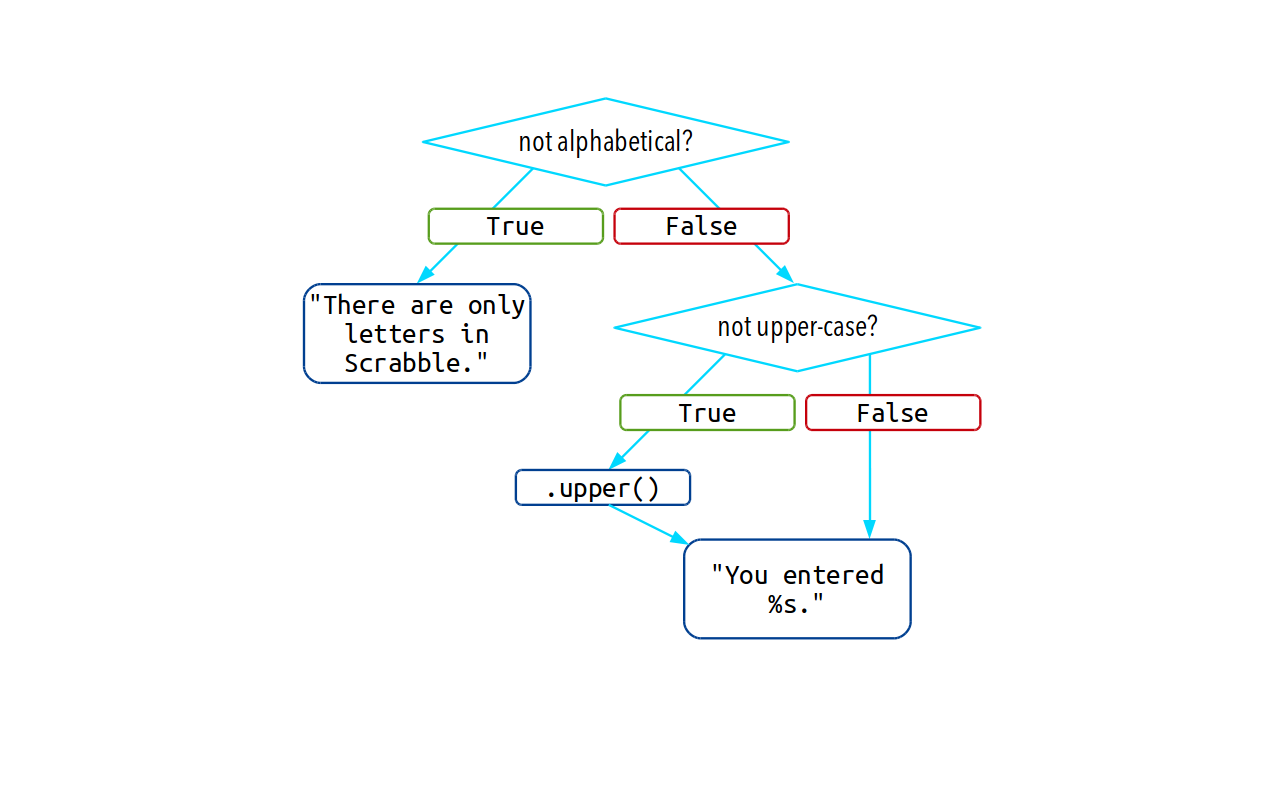
\includegraphics[width=\textwidth]{./img/control-flow-nesting-else.png}
\end{frame}

%%%%%%%%%%%%%%%%%%%%%%%%%%%%%%%%%%%%%%%%%%%%%%%%%%%%%%%%%%%%%%%%%%%%%%%%%%%%%%%%
\begin{frame}
  \frametitle{Exercise:  Nesting}
  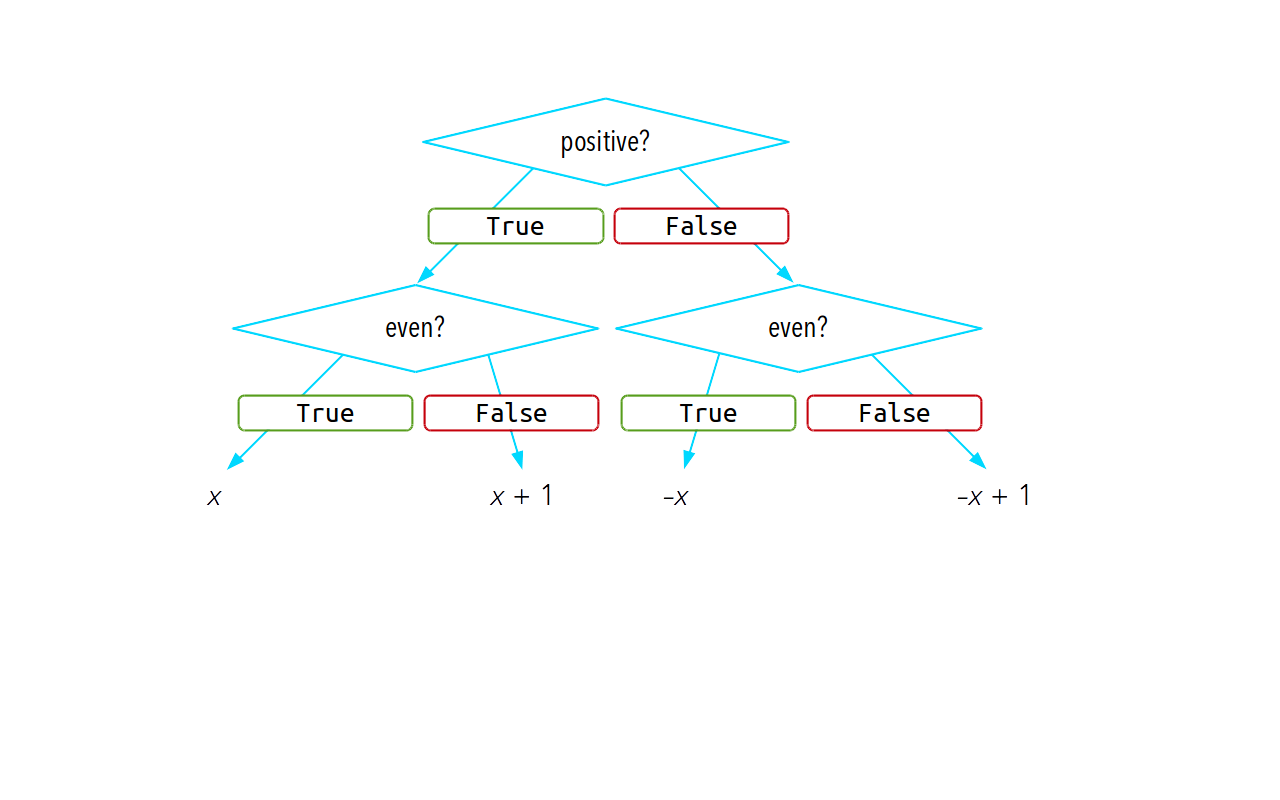
\includegraphics[width=\textwidth]{./img/control-flow-nesting-else-ex.png}
\end{frame}

%%%%%%%%%%%%%%%%%%%%%%%%%%%%%%%%%%%%%%%%%%%%%%%%%%%%%%%%%%%%%%%%%%%%%%%%%%%%%%%%
\begin{frame}[fragile]
  \frametitle{Example}
  \Enlarge

  \begin{semiverbatim}
  def evenpos(x):
if x >= 0:
    if (x%2) == 0:
        return x
    else:
        return x + 1
else:
    if (x%2) == 0:
        return -x
    else:
        return (-x) + 1
  \end{semiverbatim}
\end{frame}

%%%%%%%%%%%%%%%%%%%%%%%%%%%%%%%%%%%%%%%%%%%%%%%%%%%%%%%%%%%%%%%%%%%%%%%%%%%%%%%%
\begin{frame}[fragile]
  \frametitle{Multi-way branch}
  \Enlarge

  \begin{itemize}
  \myitem  Sometimes we need to select among many choices.
  \end{itemize}
  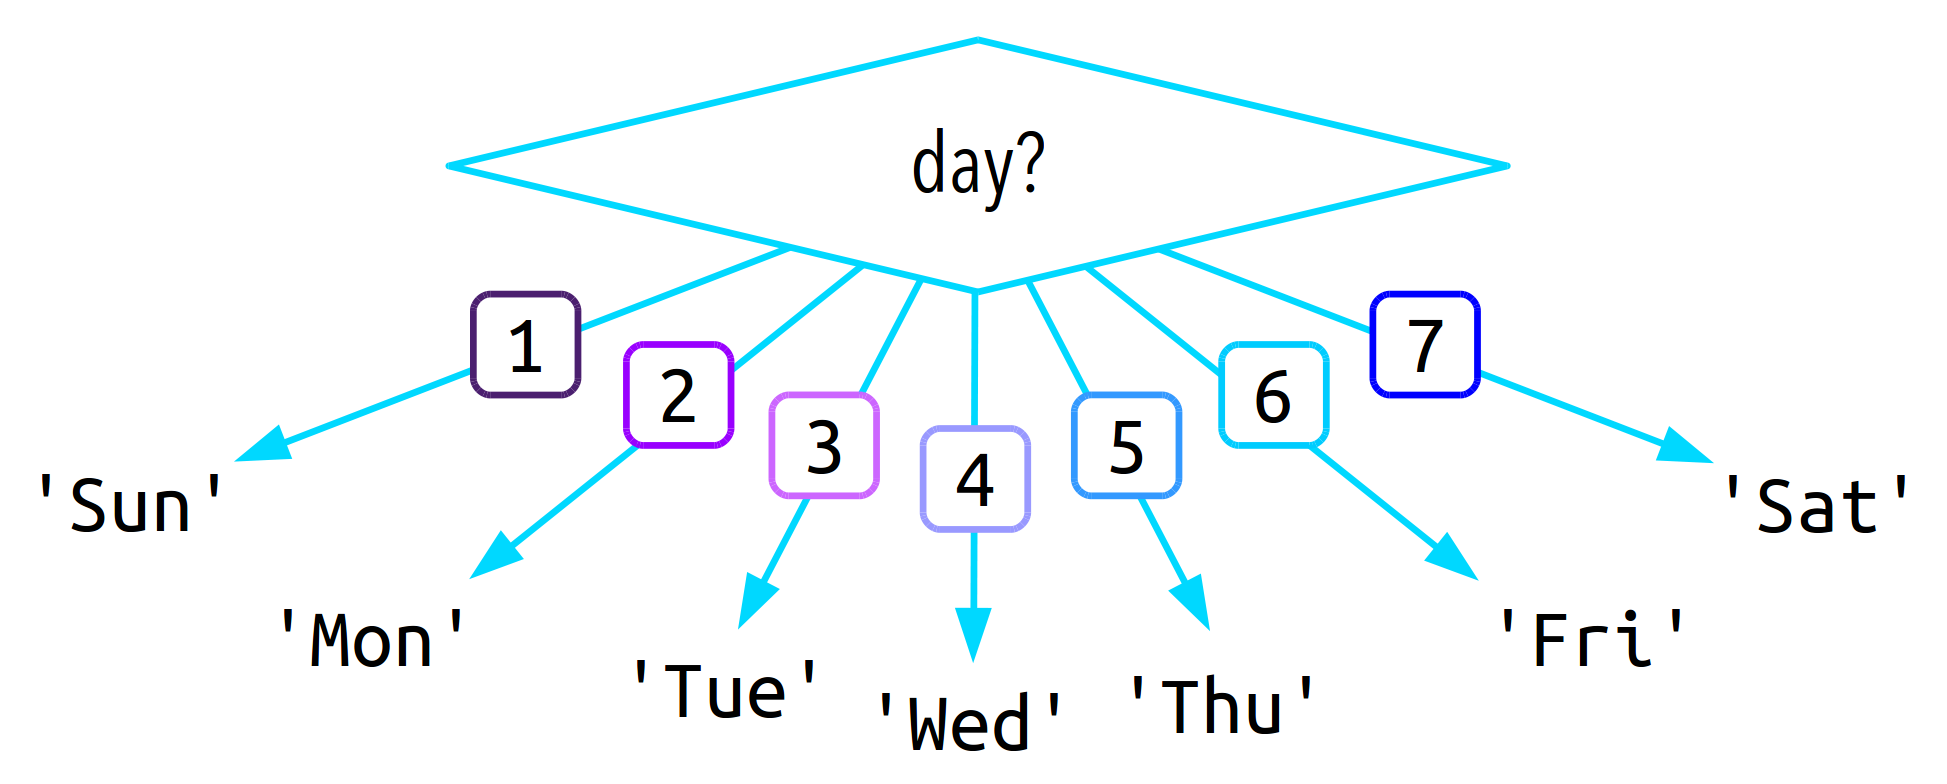
\includegraphics[width=0.8\textwidth]{./img/control-flow-multi.png}
\end{frame}

%%%%%%%%%%%%%%%%%%%%%%%%%%%%%%%%%%%%%%%%%%%%%%%%%%%%%%%%%%%%%%%%%%%%%%%%%%%%%%%%
\begin{frame}[fragile]
  \frametitle{Example}
  \Enlarge

  \begin{semiverbatim}
if day == 1:
    print("Sunday")
else:
    if day == 2:
        print("Monday")
    else:
        if day == 3:
            print("Tuesday")
        else:
            if day == 4:
                print("Wednesday")
            else:
                if day == 5:
                    print("Thursday")
                else:
                    if day == 6:
                        print("Friday")
                    else:
                        if day == 7:
                            print("Saturday")
  \end{semiverbatim}
\end{frame}

%%%%%%%%%%%%%%%%%%%%%%%%%%%%%%%%%%%%%%%%%%%%%%%%%%%%%%%%%%%%%%%%%%%%%%%%%%%%%%%%
\begin{frame}[fragile]
  \frametitle{Example}
  \Enlarge

  \begin{semiverbatim}
if day == 1:
    print("Sunday")
elif day == 2:
    print("Monday")
elif day == 3:
    print("Tuesday")
elif day == 4:
    print("Wednesday")
elif day == 5:
    print("Thursday")
elif day == 6:
    print("Friday")
elif day == 7:
    print("Saturday")
else:
    print("That is not a valid day.")
  \end{semiverbatim}
\end{frame}

%%%%%%%%%%%%%%%%%%%%%%%%%%%%%%%%%%%%%%%%%%%%%%%%%%%%%%%%%%%%%%%%%%%%%%%%%%%%%%%%
\begin{frame}[fragile]
  \frametitle{\texttt{if}/\texttt{elif}/\texttt{else} statement}
  \Enlarge

  \begin{itemize}
  \myitem  We create an \texttt{if}/\texttt{elif}/\texttt{else} statement as follows:
    \begin{itemize}
    \mysubitem  the keyword \texttt{if}
    \mysubitem  a logical comparison (results in \texttt{bool})
    \mysubitem  a \textbf{block} of code
    \mysubitem  the keyword \texttt{elif}
    \mysubitem  a logical comparison (results in \texttt{bool})
    \mysubitem  a \textbf{block} of code
    \mysubitem  the keyword \texttt{else}
    \mysubitem  a different \textbf{block} of code
    \end{itemize}
  \end{itemize}
\end{frame}

%%%%%%%%%%%%%%%%%%%%%%%%%%%%%%%%%%%%%%%%%%%%%%%%%%%%%%%%%%%%%%%%%%%%%%%%%%%%%%%%
\section{Iteration Redux}

%%%%%%%%%%%%%%%%%%%%%%%%%%%%%%%%%%%%%%%%%%%%%%%%%%%%%%%%%%%%%%%%%%%%%%%%%%%%%%%%
\begin{frame}[fragile]
  \frametitle{Example}
  \Enlarge

  \begin{semiverbatim}
colors = [ 'red', 'yellow', 'blue', 'jale', 'ulfire' ]
for color in colors:
    print( color )
  \end{semiverbatim}
\end{frame}

%%%%%%%%%%%%%%%%%%%%%%%%%%%%%%%%%%%%%%%%%%%%%%%%%%%%%%%%%%%%%%%%%%%%%%%%%%%%%%%%
\begin{frame}[fragile]
  \frametitle{\texttt{list} data type}
  \Enlarge

  \begin{itemize}
  \myitem  The \texttt{list} type represents an ordered collection of items. \pause
  \myitem  \texttt{list} is an \emph{iterable} and a \emph{container}. \pause
  \myitem  Containers hold values of any type (doesn't have to be the same).
  \end{itemize}
\end{frame}

%%%%%%%%%%%%%%%%%%%%%%%%%%%%%%%%%%%%%%%%%%%%%%%%%%%%%%%%%%%%%%%%%%%%%%%%%%%%%%%%
\begin{frame}[fragile]
  \frametitle{\texttt{list} statement}
  \Enlarge

  \begin{itemize}
  \myitem  We create a \texttt{list} as follows:
    \begin{itemize}
    \mysubitem  opening bracket \texttt{[}
    \mysubitem  one or more comma-separated data values
    \mysubitem  closing bracket \texttt{]}
    \end{itemize}
  \end{itemize}
\end{frame}

%%%%%%%%%%%%%%%%%%%%%%%%%%%%%%%%%%%%%%%%%%%%%%%%%%%%%%%%%%%%%%%%%%%%%%%%%%%%%%%%
\begin{frame}[fragile]
  \frametitle{\texttt{list} statement}
  \Enlarge

  \begin{itemize}
  \myitem  \texttt{list}s work a bit like strings:
    \begin{semiverbatim}
x = [ 10, 3.14, "Ride" ]

print( x[1] )
print( x[1:3] )
print( len(x) )

for i in x:
    print(i)
    \end{semiverbatim}
  \end{itemize}
\end{frame}

%%%%%%%%%%%%%%%%%%%%%%%%%%%%%%%%%%%%%%%%%%%%%%%%%%%%%%%%%%%%%%%%%%%%%%%%%%%%%%%%
\begin{frame}[fragile]
  \frametitle{\texttt{list} statement}
  \Enlarge

  \begin{itemize}
  \myitem  But strings are \emph{immutable} (we can't change contents without creating a new string): \pause
  \end{itemize}
  \begin{columns}
  \begin{column}{0.6\textwidth}
    \begin{semiverbatim}
s = "good advise"
s[9] = 'c'                 # nope

s = s[:9] + 'c' + s[9:]    # this way
    \end{semiverbatim}
  \end{column}
  \begin{column}{0.4\textwidth}
  ~ \\
  \textcolor{red}{$\leftarrow$ disallowed!}
  ~ \\
  \end{column}
  \end{columns}
\end{frame}

%%%%%%%%%%%%%%%%%%%%%%%%%%%%%%%%%%%%%%%%%%%%%%%%%%%%%%%%%%%%%%%%%%%%%%%%%%%%%%%%
\begin{frame}[fragile]
  \frametitle{\texttt{list} statement}
  \Enlarge

  \begin{itemize}
  \myitem  We \emph{can} change \texttt{list} content---they are \emph{mutable}. \pause
  \end{itemize}
  \begin{columns}
  \begin{column}{0.6\textwidth}
    \begin{semiverbatim}
    x = [ 4,1,2,3 ]
    x[3] = -2
    x.append(5)
    del x[1]
    x.sort()
    \end{semiverbatim}
  \end{column}
  \begin{column}{0.4\textwidth}
  ~ \\
  \textcolor{red}{$\leftarrow$ item assignment}
  ~ \\ ~ \\ ~ \\ ~ \\
  \end{column}
  \end{columns}
\end{frame}

%%%%%%%%%%%%%%%%%%%%%%%%%%%%%%%%%%%%%%%%%%%%%%%%%%%%%%%%%%%%%%%%%%%%%%%%%%%%%%%%
\begin{frame}[fragile]
  \frametitle{Example}
  \Enlarge

  \begin{semiverbatim}
for i in range(10):
    print(i ** 2)
  \end{semiverbatim}
\end{frame}

%%%%%%%%%%%%%%%%%%%%%%%%%%%%%%%%%%%%%%%%%%%%%%%%%%%%%%%%%%%%%%%%%%%%%%%%%%%%%%%%
\begin{frame}[fragile]
  \frametitle{\texttt{range} function}
  \Enlarge

  \begin{itemize}
  \myitem  The \texttt{range} function returns an \texttt{iterator} containing integers: \pause
  \myitem  \texttt{range} can be cast as a \texttt{list}. \pause
  \myitem  Two arguments:
    \begin{itemize}
    \mysubitem  (optional) the starting value of the range (inclusive)
    \mysubitem  the ending value of the range (exclusive)
    \end{itemize}
  \end{itemize}
\end{frame}

%%%%%%%%%%%%%%%%%%%%%%%%%%%%%%%%%%%%%%%%%%%%%%%%%%%%%%%%%%%%%%%%%%%%%%%%%%%%%%%%
\section{Reminders}

%%%%%%%%%%%%%%%%%%%%%%%%%%%%%%%%%%%%%%%%%%%%%%%%%%%%%%%%%%%%%%%%%%%%%%%%%%%%%%%%
\begin{frame}
  \frametitle{Reminders}
  \Enlarge

  \begin{itemize}
  \myitem  Homework \#4 is due Friday Sep.\ 23.
  \myitem  Midterm \#1 will be Monday Oct.\ 3.  (evening)
  \end{itemize}
\end{frame}

\end{document}
